%
\section{Testen}

\subsection{Testen der Methode \textit{IsWithinConstructorOf}}
In C\# 6 können Auto-Properties ohne Setter deklariert werden. C\# Essentials überprüft, ob der Setter weggelassen werden kann und teilt dies gegebenenfalls dem Benutzer mit. Die zu testende Methode \textit{IsWithinConstructorOf} überprüft dabei, ob das Setzen des Auto-Properties im Konstruktor stattfindet. Die statische Analyse ergab, dass diese Methode sehr Komplex und damit sehr fehleranfällig ist. Daher haben wir uns entschlossen diese genauer zu testen. Dazu haben wir, den in Abbildung~\ref{fig:graph-constructor} dargestellten, Kontrollflussgraphen erstellt. Anschließend haben wir folgende Testpfade für unterschiedliche Coverage Kriterien aufgestellt.\\


Node Coverage: TR = \{1, 2, 3, 4, 5, 6, 7\}\\
Example Test Paths = [1, 3, 4, 5], [1, 3, 6, 2], [1, 3, 7, 2]\\

Edge Coverage: TR = \{(1, 2), (1, 3), (3, 1), (3, 4), (4, 5), (3, 6), (6, 2), (3, 7), (7, 2)\}\\
Example Test Paths = [1, 3, 1, 2], [1, 3, 4, 5], [1, 3, 6, 2], [1, 3, 7, 2]\\

Edge Pair Coverage: TR = \{[1, 3, 1], [1, 3, 4], [1, 3, 6], [1, 3, 7], [3, 1, 3], [3, 1, 2], [3, 4, 5], [3, 6, 2], [3, 7, 2]\}\\
Example Test Paths = [1, 3, 1, 3, 1, 2], [1, 3, 4, 5], [1, 3, 6, 2], [1, 3, 7, 2]\\

Prime Path Coverage: TR = \{[1, 3, 4, 5], [1, 3, 6, 2], [1, 3, 7, 2], [3, 1, 2], [3, 1, 3], [1, 3, 1]\}
Example Test Paths: [1, 3, 1, 3, 1, 2], [1, 3, 4, 5], [1, 3, 6, 2], [1,3,7,2]\\

Zu erkennen ist, dass Edge Pair und Prime Path Coverage die selben Test Paths besitzen. 
\begin{figure}[]
	\centering
	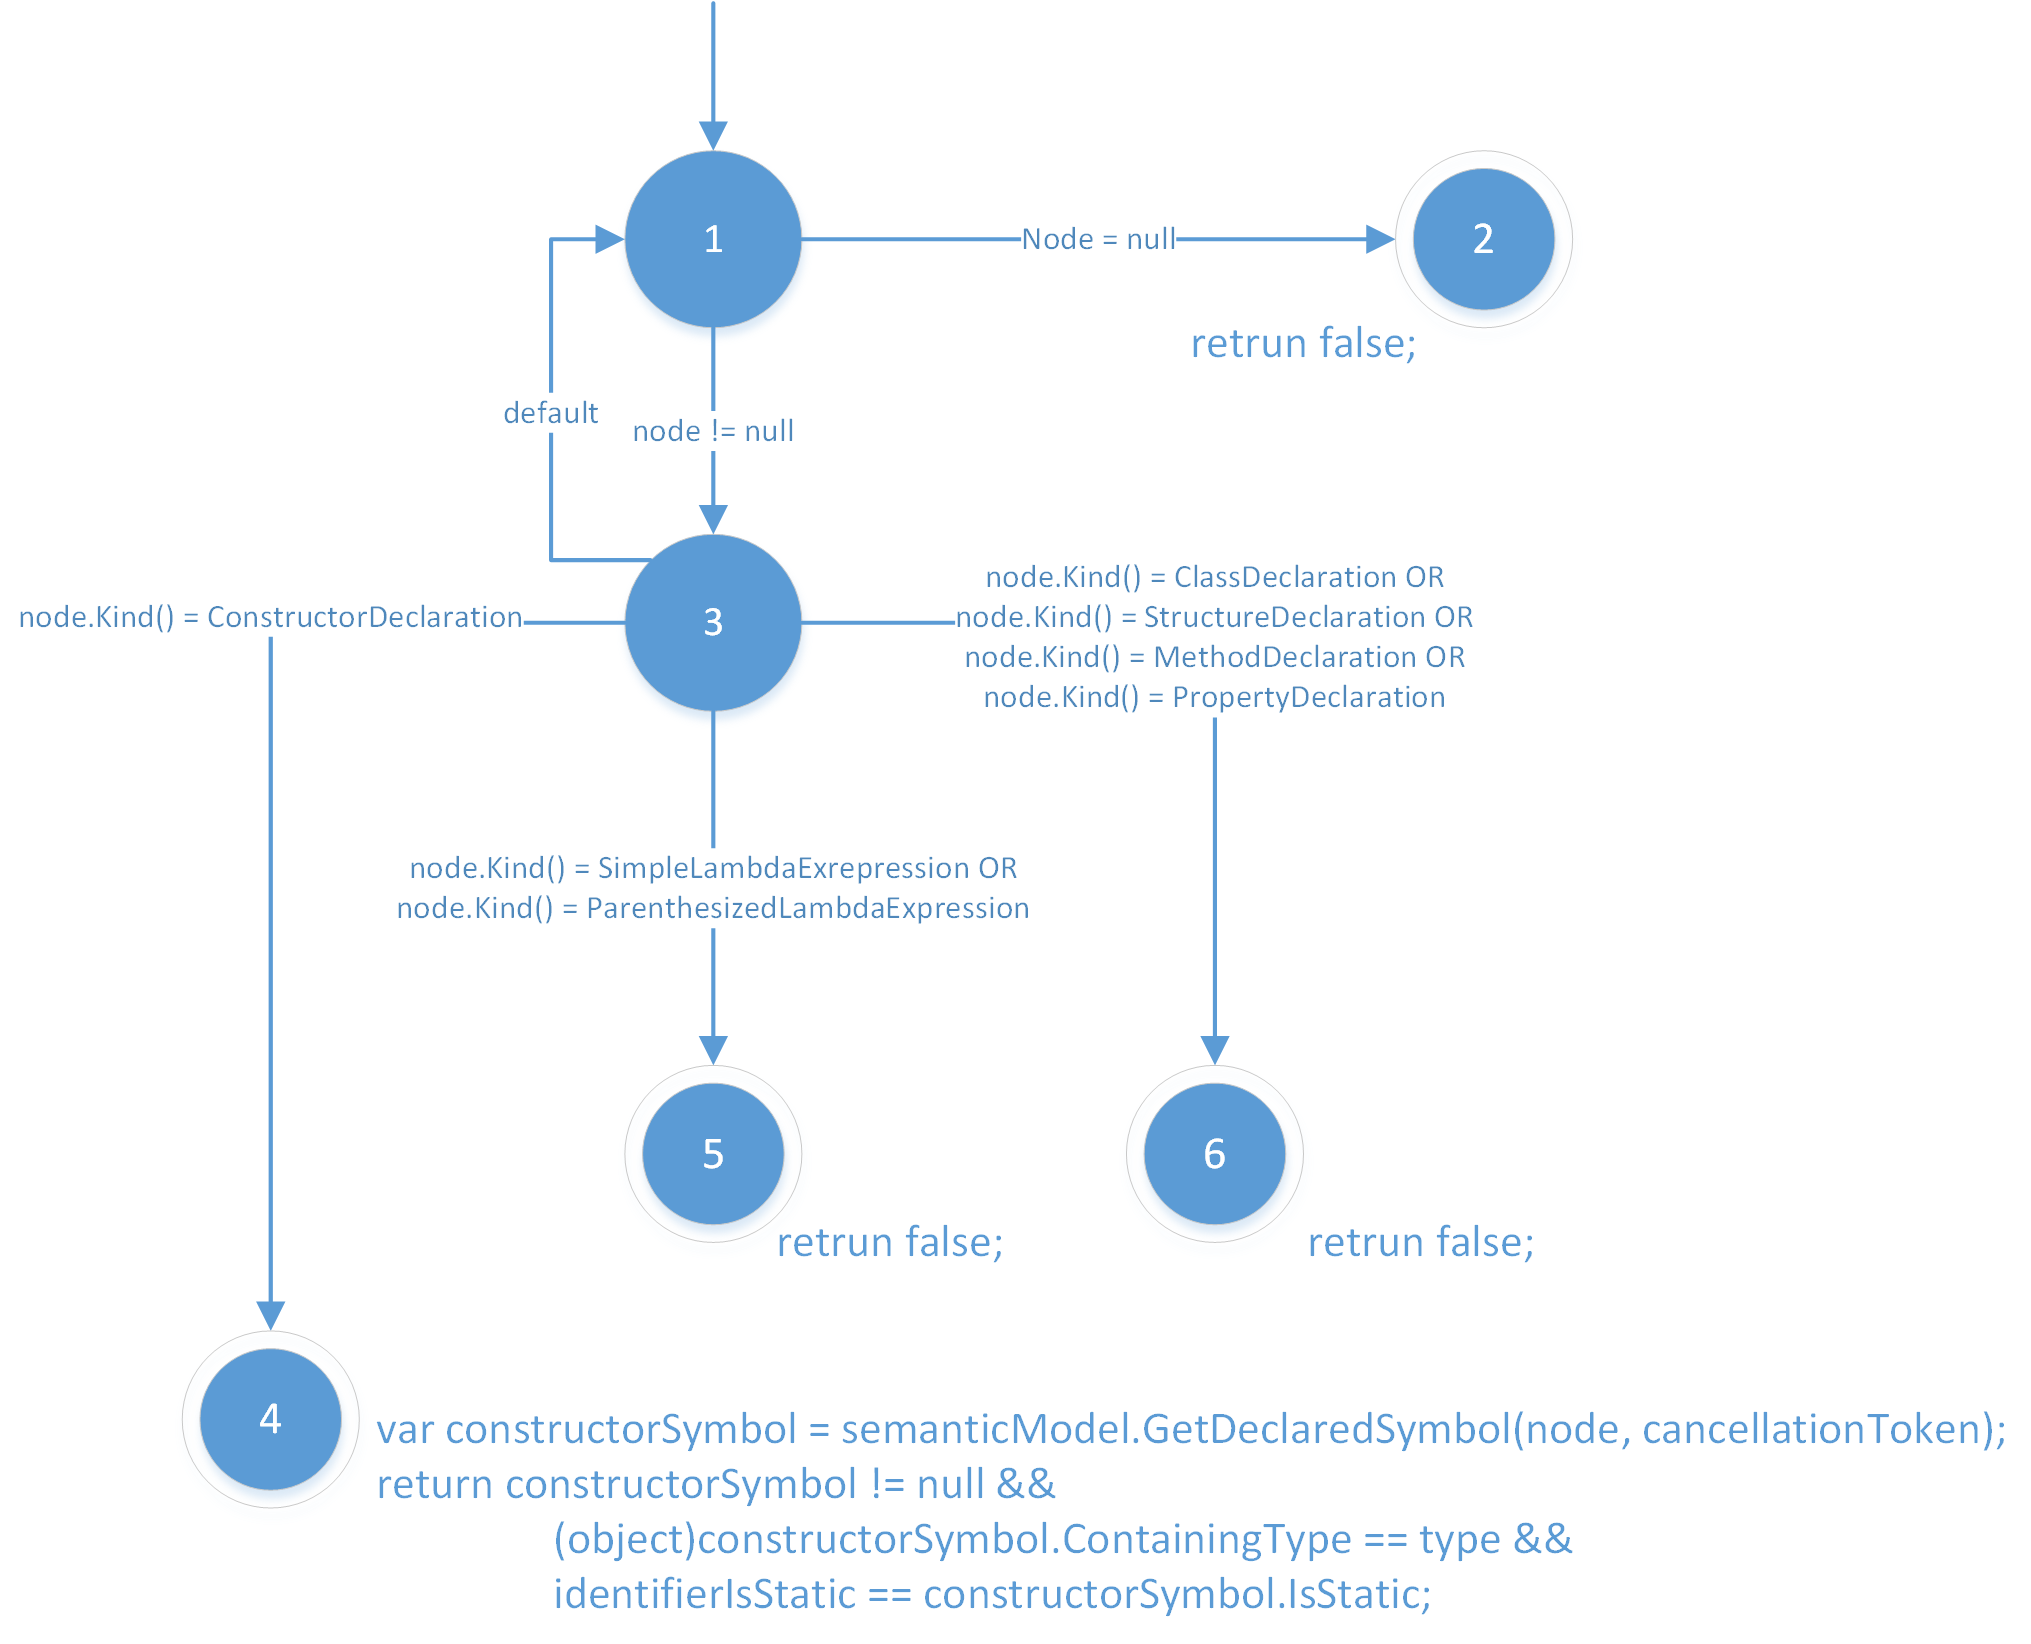
\includegraphics[width=\textwidth]{images/GraphIsWithinConstructorOf.png}
	\caption{Graph für die Methode \textit{IsWithinConstructorOf}()}
	\label{fig:graph-constructor}
\end{figure}


\begin{figure}[]
	\centering
	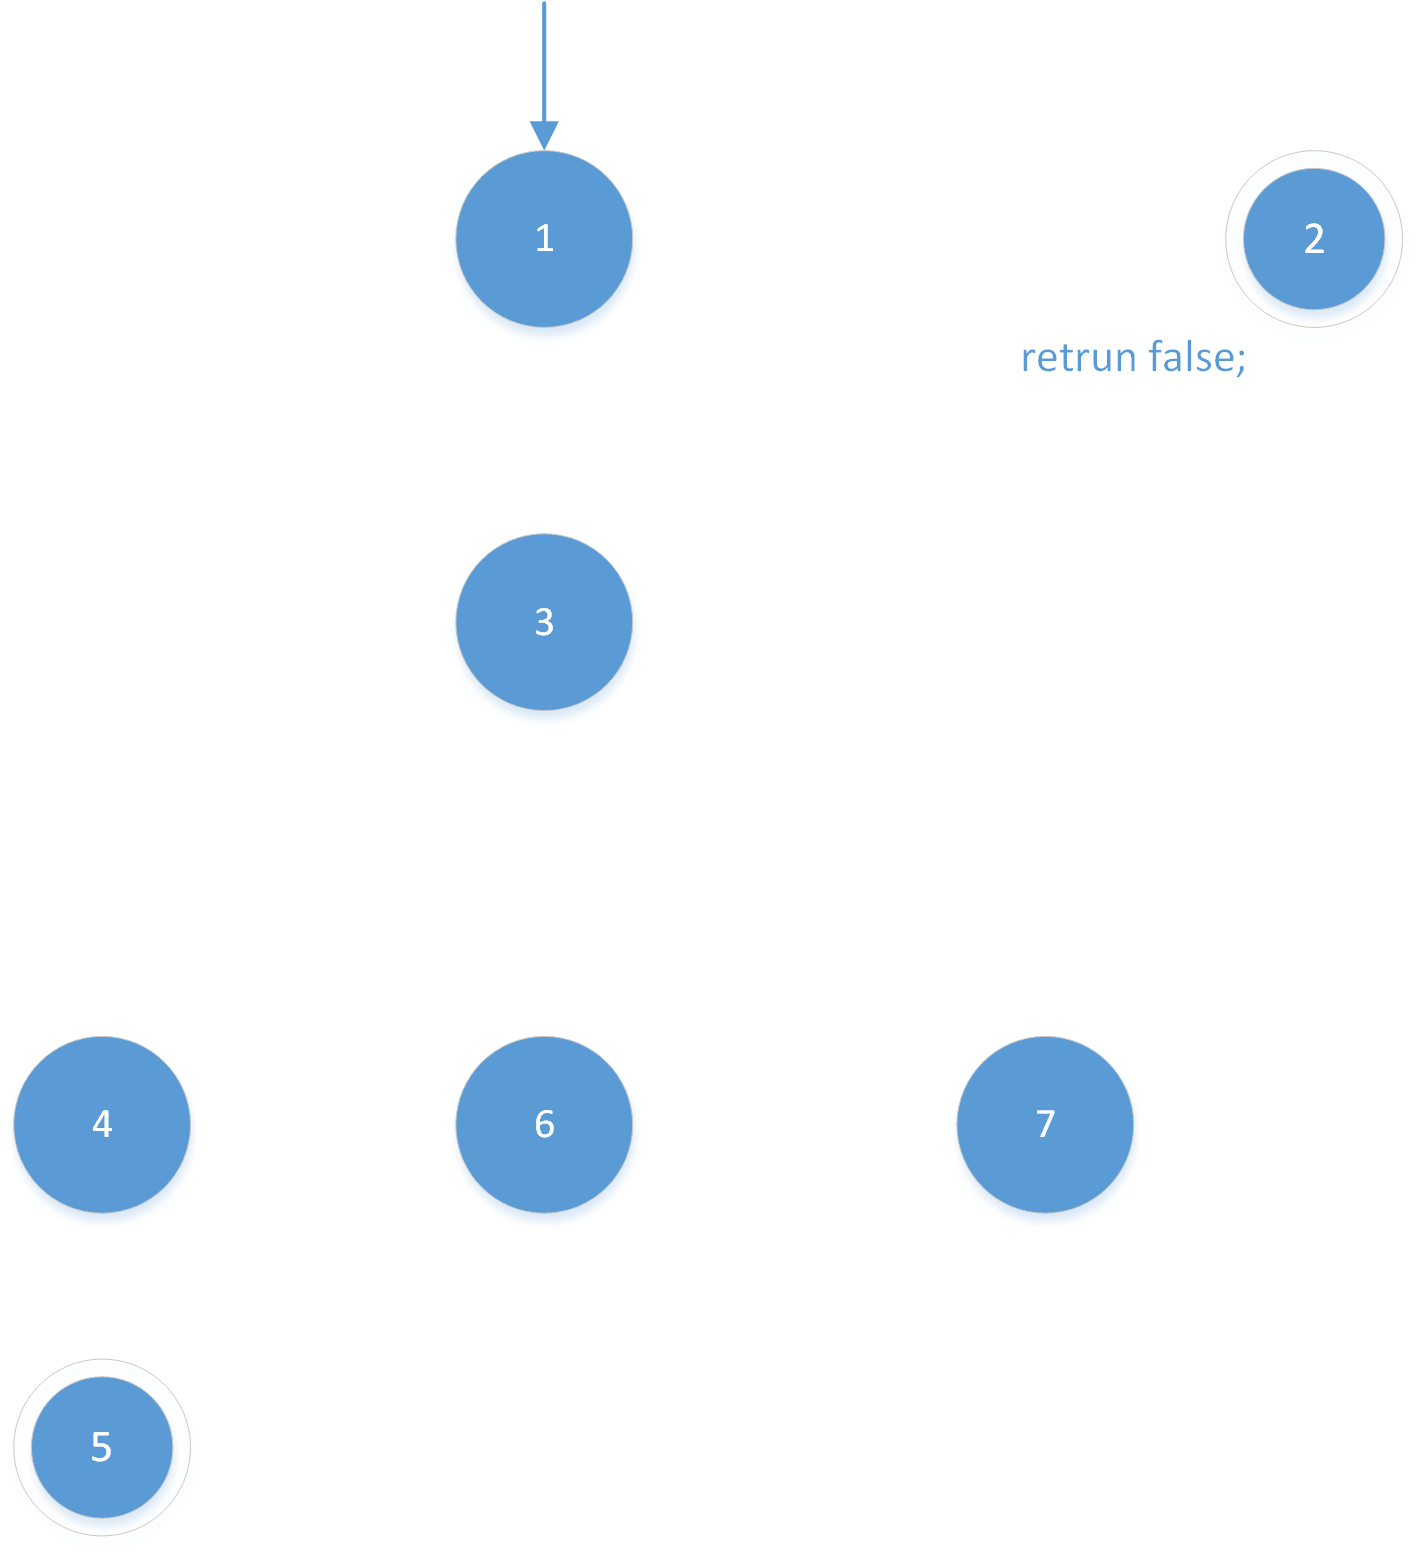
\includegraphics[width=\textwidth]{images/GraphCreateInterpolatedString.png}
	\caption{Graph für die Methode \textit{CreateInterpolatedString}()}
	\label{fig:graph-interpolatedstring}
\end{figure}